\documentclass{article} % For LaTeX2e
\usepackage[submission]{colm2026_conference}

\usepackage{microtype}
\usepackage{url}
\usepackage{booktabs}
\usepackage{multirow}
\usepackage{amsmath}
\usepackage{amssymb}
\usepackage{xcolor}
\usepackage{graphicx}
\usepackage{float}
\usepackage{tikz}
\usepackage{pgfplots}
\usepackage{listings}
\usepackage{hyperref}
\pgfplotsset{compat=1.17}
\usetikzlibrary{positioning, arrows.meta, fit, backgrounds}

\usepackage{lineno}

\definecolor{darkblue}{rgb}{0, 0, 0.5}
\definecolor{sbred}{rgb}{0.78, 0.10, 0.10}
\definecolor{sbblue}{rgb}{0.13, 0.36, 0.62}
\definecolor{sbgreen}{rgb}{0.18, 0.49, 0.20}
\definecolor{sborange}{rgb}{0.85, 0.45, 0.10}
\hypersetup{colorlinks=true, citecolor=darkblue, linkcolor=darkblue, urlcolor=darkblue}

\newcommand{\salesbench}{\textsc{SalesBench}}
\newcommand{\tool}[1]{\texttt{#1}}
\setlength{\emergencystretch}{3em}

% Compact, monochrome style for rollout-trace listings (Figure 3).
\lstdefinestyle{trace}{
  basicstyle=\ttfamily\scriptsize,
  breaklines=true,
  breakindent=14pt,
  columns=fullflexible,
  keepspaces=true,
  showstringspaces=false,
  frame=single,
  framesep=4pt,
  xleftmargin=2pt,
  xrightmargin=2pt,
  rulecolor=\color{black!30},
  backgroundcolor=\color{black!3},
  aboveskip=3pt,
  belowskip=2pt,
}

\title{\salesbench{}: A Long-Horizon, Agent-to-Agent Benchmark\\ for Tool-Use Agent Behavior}

\author{Anonymous authors\\Paper under double-blind review}

\begin{document}

\ifcolmsubmission
\linenumbers
\fi

\maketitle

\begin{abstract}
Most agent benchmarks ask \emph{what} an agent achieves against a static rubric or fixed
verifier. For deployed agents, an equally important question is \emph{how} they behave:
how they allocate a budget, where they break, whether they remain compliant under
optimization pressure, and whether a learned policy survives a counterparty it did not
train against. We introduce \salesbench{}, a long-horizon, agent-to-agent benchmark for
measuring those behaviors. A seller agent operates inside a deterministic insurance-sales
simulator with ${\sim}100$ procedurally generated leads and a fixed time budget. It must
maximize converted monthly recurring revenue by searching a customer database, quoting plans, placing
calls, and closing deals, while a separate buyer language model, instantiated with one of
ten personality archetypes, decides whether to accept, reject, or hang up. Because the
world is a deterministic state machine, variance comes from the seller and buyer models;
seller mistakes are separated from buyer-model failures; and four buyer-prompt variants
turn counterparty overfitting into a quantitative test. We use \salesbench{} as both a
training signal and an evaluation suite, training a 2B-parameter model with online
reinforcement learning and analyzing its behavior. The trained policy learns in two phases, tool-interface mastery
then selling skill, and at full scale is productive but brittle: it converts ${\sim}18$ leads using only
${\sim}11\%$ of the time budget before terminating on the invalid-action ceiling rather than on time. Compliance holds
under revenue optimization (do-not-call violations stay near zero), and the policy transfers to three unseen buyer
decision styles ($8\text{--}20\%$ per-lead conversion), degrading less than the base model as the pipeline doubles.
Finally, reward shaping is fragile under RL: auxiliary terms become floor strategies once the model can collect them
without selling. We release the environment, curriculum, behavioral instrumentation, and harness.
\end{abstract}

\section{Introduction}

Language-model agents are deployed on tasks where success is not a single correct answer
but the cumulative outcome of many decisions made under a budget. A coding agent navigates
a repository across dozens of tool calls; a research agent reads, synthesizes, and revises;
a customer-facing agent negotiates across a multi-turn conversation. Yet many agent
benchmarks retain the shape of question answering: a prompt, a trajectory, and a verifier
that scores the trajectory against a fixed target \citep{liu2024agentbench, mialon2024gaia}.
This format is convenient because it is deterministic and gradeable, but it mostly measures
\emph{what} an agent achieves. It says less about \emph{how} the result was produced, which is
the process question that determines whether an agent is robust, compliant, and useful under
deployment pressure.

We build on a line that evaluates agents through a behavioral lens
\citep{park2023generative, zhou2024sotopia, pan2023machiavelli}: evaluating the
\emph{behavior} of an agent requires two ingredients that single-trajectory benchmarks often omit.
The first is \textbf{horizon under a hard budget}. A real agent does not get an arbitrary
number of actions; it has a finite amount of time, money, context, or tolerance for error,
and good behavior means \emph{allocating} that budget, deciding which leads to pursue, when
to stop talking and act, and when to cut losses. The second is the \textbf{agent-to-agent}
structure. The environment is not a passive grader but another adaptive agent with its own
goals, information, and personality, whose responses the protagonist cannot dictate and must
instead influence. Sales, negotiation, tutoring, and customer support all have this structure,
and all are domains where current models are being deployed with little principled measurement
of how they behave under pressure.

Existing benchmarks tend to supply one ingredient but not both: long-horizon business simulators are stateful and
budgeted but pair the agent with scripted customers, while tool-agent-user benchmarks supply an adaptive
counterparty in shorter episodes. \salesbench{} sits at the intersection: long-horizon, stateful, budgeted,
driven by an adaptive language-model counterparty, and graded by a verifiable outcome read directly from
environment state, namely whether a deal closed and at what premium.

We introduce \salesbench{}, a benchmark that captures both ingredients in a single reproducible task, simulated
insurance sales (\S\ref{sec:env}). A seller agent works a pool of ${\sim}100$ prospective buyers (``leads'') under a
hard budget of, e.g., $50$ simulated working hours, spending simulated minutes on each action (searching a
customer-relationship-management (CRM) system, pulling a quote, starting a call, proposing an offer) to maximize
converted monthly recurring revenue (MRR), the sum of premiums on deals it closes. Closing requires a separate buyer
language model, instantiated per-lead with one of ten personality archetypes (Analytical, Skeptic, Budget Hawk,
Protector, and so on) and a ``temperature'' from cold to hot, to accept the offer; the buyer decides, in character,
whether to accept, reject, or hang up.

This design yields three properties a behavioral benchmark should have. \textbf{Reproducible world, stochastic
agents}: the simulator (\S\ref{sec:env}) is a deterministic state machine with zero model calls, so for a fixed seed
the only variance is the seller and buyer models, which makes $k$-rollout behavioral comparison meaningful.
\textbf{Failure attribution}: \salesbench{} separates a protagonist's bad decisions from counterparty-model failures
(\S\ref{sec:attribution}), penalizing seller errors while resolving buyer-model failures to a benign rejection.
\textbf{A built-in generalization axis}: four buyer-prompt variants share identical information but differ in decision
style, so an agent trained against one can be tested against the other three.

To show the benchmark is a trainable signal rather than only a static evaluation set, we run a four-stage
difficulty curriculum (2, 4, 8, then 20 leads) that trains a 2B-parameter model with online
reinforcement learning against the \textsc{Default} buyer, then evaluate it at full scale (50 and 100
leads) against all four buyers (\S\ref{sec:experiments}). Rather than reporting a single capability
number, we use the run to surface the behaviors the benchmark is meant to measure:
\begin{itemize}
\itemsep0.15em
\item \textbf{Two-phase learning.} The agent first masters the tool \emph{interface} (schema errors
fall sharply at small scale), and only then, much more slowly, learns the \emph{skill} of closing:
fitting coverage to budget and triaging which leads to pursue (\S\ref{sec:dynamics}).
\item \textbf{A brittleness signature.} At 100 leads the trained agent uses only ${\sim}11\%$ of its time budget:
it converts ${\sim}18$ leads and then trips a mistake ceiling, because interface discipline learned at small scale
does not fully transfer to the long horizon (\S\ref{sec:behavior}).
\item \textbf{Compliance under optimization.} Do-not-call violations stay near zero even as the agent is optimized
hard for revenue (\S\ref{sec:behavior}).
\item \textbf{Counterparty-style generalization.} Trained only against \textsc{Default}, the agent sustains
$8\text{--}20\%$ per-lead conversion against all four buyer styles, including three it never saw. This suggests a
transferable policy, not counterparty overfitting (\S\ref{sec:scaling}).
\item \textbf{Reward-shaping fragility.} Almost any auxiliary reward term becomes a floor trap once the model can
collect it without selling, so \salesbench{} doubles as a testbed for reward-hacking behavior (\S\ref{sec:discussion}).
\end{itemize}

Our contributions are: (1) \salesbench{}, a reproducible long-horizon agent-to-agent benchmark for
\emph{measuring tool-use agent behavior}, with explicit seller/buyer failure attribution and a buyer-style
generalization axis; (2) a deterministic simulator, ten-archetype buyer model, revenue-first reward,
difficulty curriculum, and zero-weight behavioral instruments for termination attribution, pipeline triage, and
per-counterparty conversion fingerprints; (3) a behavioral characterization of a small RL-trained agent:
two-phase learning, an error-ceiling brittleness signature, compliance under optimization, and counterparty-style
transfer.

\section{Related work}

\paragraph{Agentic and tool-use benchmarks.} A growing body of work evaluates language models as agents that call
tools over multiple turns: AgentBench \citep{liu2024agentbench} and GAIA \citep{mialon2024gaia} aggregate diverse
tasks; ToolLLM \citep{qin2024toolllm} and Gorilla \citep{patil2024gorilla} target API invocation; WebArena,
SWE-bench, and TheAgentCompany \citep{zhou2024webarena, jimenez2024swebench, xu2024theagentcompany} study realistic
web, software, and professional environments. These are mostly graded against a static target (a gold trajectory, a
passing test suite, or a reachable goal), and even analytical multi-turn boards such as AgentBoard
\citep{ma2024agentboard} score progress against fixed tasks. \salesbench{} instead uses an adaptive counterparty, a
continuous resource-allocation outcome, and rollout instrumentation for studying \emph{how} the policy behaves.

\paragraph{Agent behavior and social simulation.} A complementary line studies agents through a behavioral lens:
Generative Agents \citep{park2023generative} and Concordia \citep{vezhnevets2023concordia} simulate language-model
personas; SOTOPIA \citep{zhou2024sotopia} evaluates social intelligence in agent-to-agent episodes; MACHIAVELLI
\citep{pan2023machiavelli} measures the reward-versus-ethics trade-off; and model-written evaluations
\citep{perez2022discovering} and sycophancy \citep{sharma2024sycophancy} surface emergent behaviors induced by
optimization. \salesbench{} adds a long-horizon, economically grounded setting where budget allocation, compliance
under pressure, counterparty influence, and brittleness are read directly from a deterministic environment rather
than a judge.

\paragraph{Agent-to-agent and tool-agent-user simulation.} The closest line of work simulates a second agent as part
of the environment: $\tau$-bench and $\tau^2$-bench \citep{yao2024taubench, barres2025tau2bench} introduce a
user-simulator language model the agent must serve under domain policies, with the three-party structure (agent,
simulated user, environment) we adopt. \salesbench{} shares this pattern but targets a different regime: the
counterparty can reject or hang up, the objective is competitive revenue maximization rather than policy-compliant
completion, and the horizon spans hundreds of tool calls across ${\sim}100$ counterparties under one budget.
Negotiation and persuasion \citep{lewis2017deal, wang2019persuasion, bakhtin2022cicero} study influence inside a single
conversation; \salesbench{} embeds many such conversations in a portfolio-level budgeting problem.

\paragraph{Long-horizon, budgeted agents.} Vending-Bench \citep{backlund2025vending} runs a simulated business over
long horizons with persistent state and a budget, closest to ours in operational shape, but its customers are scripted,
whereas $\tau$-bench's counterparty is adaptive but its episodes are short. \salesbench{} occupies the intersection:
long-horizon, stateful, adaptive-counterparty, resource-constrained, and graded by a verifiable state-derived outcome
with no judge.

\paragraph{Reinforcement learning and behavioral intervention.} Reinforcement learning from verifiable rewards has
driven progress in reasoning and instruction following \citep{shao2024deepseekmath, lambert2024tulu3}; we extend it to
a long-horizon, agent-to-agent task with GRPO \citep{shao2024deepseekmath} and a difficulty curriculum
\citep{bengio2009curriculum}. We treat RL post-training as a \emph{behavioral intervention}: it installs an operational
selling policy but also exposes reward-shaping fragility, a concrete instance of reward misspecification and reward
hacking \citep{pan2022reward, skalse2022reward, krakovna2020specification, pan2024feedback}. The environment is built
on \textsc{Verifiers} \citep{brown2025verifiers}, whose stateful tool-environment abstraction supports the per-rollout
simulator state and hidden tool arguments we require.

\begin{figure}[t]
\centering
\resizebox{\linewidth}{!}{%
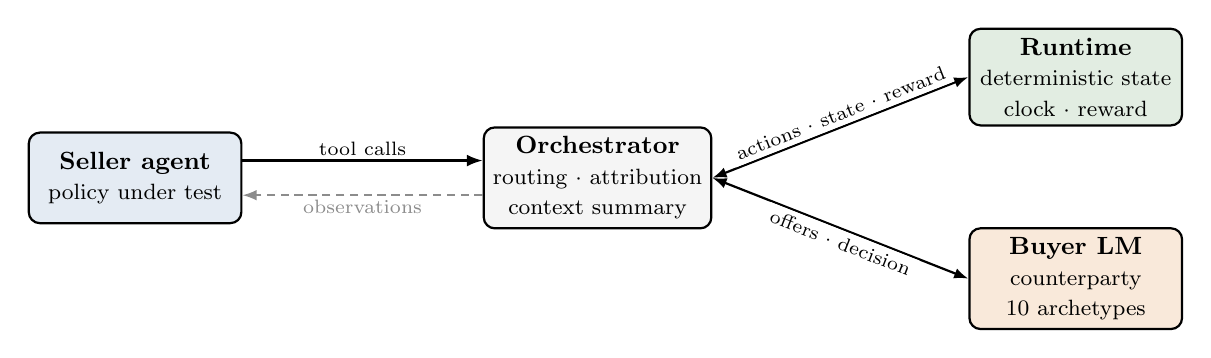
\begin{tikzpicture}[
  font=\small,
  box/.style={draw, rounded corners, align=center, minimum height=1.15cm, minimum width=2.7cm, thick},
  seller/.style={box, fill=sbblue!12},
  orch/.style={box, fill=black!4},
  rt/.style={box, fill=sbgreen!14},
  buyer/.style={box, fill=sborange!16},
  fwd/.style={draw, -{Latex[length=2mm]}, thick},
  ret/.style={draw, -{Latex[length=1.8mm]}, semithick, black!45, densely dashed},
  bi/.style={draw, {Latex[length=1.8mm]}-{Latex[length=1.8mm]}, thick},
  lab/.style={font=\scriptsize, inner sep=1.6pt},
  slab/.style={font=\scriptsize, inner sep=2pt, fill=white},
]
  \node[seller] (seller) {\textbf{Seller agent}\\\footnotesize policy under test};
  \node[orch, right=3.05cm of seller] (orch) {\textbf{Orchestrator}\\\footnotesize routing $\cdot$ attribution\\\footnotesize context summary};
  \node[rt, right=3.25cm of orch, yshift=1.28cm] (rt) {\textbf{Runtime}\\\footnotesize deterministic state\\\footnotesize clock $\cdot$ reward};
  \node[buyer, right=3.25cm of orch, yshift=-1.28cm] (buyer) {\textbf{Buyer LM}\\\footnotesize counterparty\\\footnotesize 10 archetypes};

  % Seller <-> Orchestrator: linear dialogue (two stacked arrows).
  \draw[fwd] ([yshift=2.2mm]seller.east) -- node[lab, above] {tool calls} ([yshift=2.2mm]orch.west);
  \draw[ret] ([yshift=-2.2mm]orch.west) -- node[lab, below] {observations} ([yshift=-2.2mm]seller.east);

  % Orchestrator <-> Runtime and Buyer: one bidirectional link each (clean fork).
  \draw[bi] (orch.east) -- node[slab, sloped, above, pos=0.52] {actions $\cdot$ state $\cdot$ reward} (rt.west);
  \draw[bi] (orch.east) -- node[slab, sloped, below, pos=0.52] {offers $\cdot$ decision} (buyer.west);
\end{tikzpicture}}
\caption{Three-party orchestration (the released harness). The seller agent talks only to the orchestrator,
exchanging tool calls and observations. The orchestrator applies validated actions to a deterministic runtime and
routes proposed offers to a buyer language model, then injects the buyer's decision and speech back into the
conversation. Seller errors are penalized and increment the invalid-action counter; buyer-model failures are
isolated and resolve to a benign rejection (\S\ref{sec:attribution}).}
\label{fig:orchestration}
\end{figure}

\section{The \salesbench{} environment}
\label{sec:env}

\subsection{Task and objective}
An episode places a seller agent in a sales pipeline defined by a seed; it receives a brief and a tool set, then acts
turn by turn until termination. The world is a population of $N$ leads (default $N{=}100$), a catalog of four
insurance plan types, a wall clock with budget $B = H\times 60$ (default $H{=}50$ hours, $B{=}3000$ minutes), a
per-action time-cost schedule, and a hard cap on accumulated invalid actions (default $12$). Revenue accrues only
when the buyer accepts an offer, adding the accepted premium $p_i$ to MRR. A lead's monthly budget $b_i$ is not a
hard cap: whether an over-budget offer is accepted depends on archetype and temperature, so pricing to budget is
a learned skill. The episode ends when \emph{any} budget is exhausted: time, pipeline (all leads converted, on
the do-not-call list, or out of attempts), or the mistake budget (invalid-action cap). Which budget
binds is itself a behavioral outcome we measure (\S\ref{sec:behavior}).

\subsection{Three-party orchestration}
\salesbench{} follows the agent-counterparty-environment decomposition of $\tau^2$-bench
\citep{barres2025tau2bench}, separated into three components with disjoint responsibilities
(Figure~\ref{fig:orchestration}). The \textbf{runtime} is a pure Python state machine that owns all episode
state, leads, clock, active call, callbacks, statistics, and termination, and contains zero model calls.
Determinism is enforced at construction (a single seeded RNG produces the lead population; prices are
closed-form), and we verify reproducibility (\S\ref{app:determinism}). The \textbf{buyer policy} is a separate
language model: on each proposed offer it is prompted with
the lead's full persona and the call transcript and returns a structured decision in
$\{$accept, reject, hang\_up$\}$ with a natural-language reason; during conversation it replies in character.
The \textbf{orchestrator} routes the seller's tool calls into the runtime, injects the buyer's decision and
speech back into the conversation, manages context length, enforces failure attribution, and instantiates one
buyer policy per episode. The buyer is injected into the offer tool via hidden arguments, so the seller's tool schema never
exposes the runtime or the buyer handle.

\subsection{Leads, archetypes, and pricing}
\label{sec:leads}
Leads are sampled from three demographic segments with correlated income, household size, and risk. Each lead
draws a temperature (cold/lukewarm/warm/hot; near-uniform) that shifts trust and call tolerance, and one of ten
buyer archetypes (Analytical, Skeptic, Budget Hawk, Protector, Impulse Decider, $\dots$; uniform) that sets which
of seven sales-quality criteria (discovery, tailoring, objection handling, pressure calibration, value
articulation, rapport, pacing) the buyer weights when evaluating an offer. A lead's monthly budget is a fraction
of its income drawn from a wide range, giving an even spread of deal sizes (in a representative 100-lead episode,
budgets span \$52--\$952/month, max achievable MRR \$32{,}610). The catalog prices four plan types with a
deterministic premium modulated by age, risk class, term, and smoking status, posing a real coverage-to-budget
fitting problem (\S\ref{app:pricing}).

\subsection{Tools and the canonical workflow}
The seller is given eleven tools across four namespaces, CRM, calling, products, and calendar (full list and
per-action time costs in \S\ref{app:pricing}). A productive call follows the pattern: start a call, briefly
discover the need, pull a quote that fits the budget, propose the offer, end the call. Two invariants make the
task honest: exactly one call may be active at a time, and \tool{propose\_offer} is rejected as an invalid action
unless the agent has already pulled a quote for that lead (an anti-hallucination rail against fabricated prices).
Proposing an offer costs the most time (four minutes), so the budget forces triage: the agent cannot call every
lead, and long conversations crowd out closes.

\subsection{Reward}
\label{sec:reward}
The reward is a revenue-first weighted composite computed at episode end:
\begin{equation*}
\begin{aligned}
R = {} & 1.00\cdot\frac{\mathrm{MRR}}{\mathrm{MRR}_{\max}} + 0.10\cdot\frac{\text{conversions}}{N}
  + 0.30\cdot\text{budget\_util} + 0.02\cdot\text{completion} \\
  & {}- 0.30\cdot\text{dnc\_violations} - 0.05\cdot(0.1\cdot\text{invalid\_actions}),
\end{aligned}
\end{equation*}
where $\mathrm{MRR}_{\max}$ is the sum of lead budgets, budget\_util rewards capturing a high share of each
converted lead's budget, and the penalties cover compliance and malformed actions (full definitions in
\S\ref{app:reward}). Revenue dominates by design; the shaping terms are deliberately small (an earlier, larger completion bonus induced
a degenerate floor strategy under GRPO, \S\ref{sec:discussion}). All six weights are configurable, and the
environment also logs ${\sim}35$ zero-weight diagnostic metrics plus the behavioral instruments of
\S\ref{sec:instrumentation}, so the reward and its telemetry are experimental variables.

\subsection{Failure attribution}
\label{sec:attribution}
The orchestrator separates two failure classes so that scores reflect the agent's decisions, not the buyer's
serving reliability. Seller errors (no active call, proposing without a quote, unknown plan type, calling a
do-not-call lead) raise a deterministic error and increment the invalid-action counter; buyer-model failures
(timeouts, malformed JSON, transport errors) are caught and resolved to a benign rejection, never counted against
the seller. The offer tool enforces this by ordering record-offer (seller-attributable) $\rightarrow$ call-buyer
(isolated) $\rightarrow$ apply-decision, so a buyer outage cannot manufacture an invalid action.

\subsection{Behavioral instrumentation}
\label{sec:instrumentation}
Because the central question is \emph{how} the agent behaves, the environment ships zero-weight instruments
(no reward impact) that decompose each episode at termination: (i) \emph{termination attribution}, the fraction
of episodes ending via pipeline exhaustion, time exhaustion, the invalid-action ceiling, or no controlled stop
at all; (ii) \emph{pipeline triage}, the fraction of the lead pool contacted, and the warm/hot share among
contacted leads (the pool is ${\sim}51\%$ warm/hot, so a higher share indicates the agent triages toward readier
leads); and (iii) \emph{per-counterparty conversion fingerprints}, conversion rate broken out by each of the ten
archetypes and four temperatures. These instruments turn coarse outcomes into behavioral profiles and are what
let us, in \S\ref{sec:behavior}, distinguish ``the agent ran out of time'' from ``the agent broke.''

\subsection{Context management for long horizons}
\label{sec:context}
At full scale an episode spans hundreds of tool calls and outgrows the context window, where models also degrade on
information buried in the middle of long contexts \citep{liu2024lostmiddle}. \salesbench{} compresses
deterministically: when the prompt reaches a configurable fraction (default $80\%$) of the maximum sequence
length, the orchestrator replaces older messages with a compact summary rendered from runtime state, keeping the
system prompt, briefing, and most recent messages verbatim (\S\ref{app:context}). The summary uses no model call
and fires a handful of times per episode, keeping the key-value cache stable for training. This compression is
load-bearing at 100 leads (\S\ref{sec:behavior}).

\section{Experiments}
\label{sec:experiments}
We use \salesbench{} both as a training signal and as an evaluation suite, to demonstrate the full loop the
benchmark is designed to support and to read off the agent's behavior.

\subsection{Setup}
\textbf{Curriculum.} We train a 2B-parameter base model (Qwen3.5-2B) with Group Relative Policy Optimization (GRPO)
\citep{shao2024deepseekmath} over four difficulty stages of increasing scale: 2 leads / 1 hour, 4 / 2 hours, 8 / 4
hours, and 20 / 10 hours. Only the first stage trains from scratch (to acquire the
search$\rightarrow$call$\rightarrow$quote$\rightarrow$propose workflow); each subsequent stage warm-starts from the
previous checkpoint. Training uses the \textsc{Default} buyer exclusively, $32$ rollouts per example for
group-relative advantages, online difficulty filtering, and sampling temperature $1.0$; the buyer model is a small
hosted model held fixed throughout (full hyperparameters in \S\ref{app:training}).

\textbf{Evaluation.} We evaluate at full scale, 50 and 100 leads, which is $2.5\text{--}5\times$ larger than any
training stage. Each evaluation cell rolls out $64$ episodes from the held-out evaluation split (a 128-seed split
disjoint from training), one rollout each, with deterministic context compression at threshold $0.85$ and maximum
sequence length $16{,}000$ tokens. Because each episode uses a distinct seed, the 64 episodes per cell are
independent draws; we report the standard error of the mean (SEM), the sample standard deviation across episodes
divided by $\sqrt{64}$, as $\pm$ values in Table~\ref{tab:matrix} and error bars in Figure~\ref{fig:scaling}. We run
the trained agent and the untrained base against all four buyer variants (\textsc{Default}, \textsc{Skeptical},
\textsc{Impulsive}, \textsc{Analytical}); the latter three are never seen in training. We report composite reward,
per-lead conversion rate (conv/lead), captured MRR fraction (mrr-cap), and the fraction of episodes that reach a
controlled runtime stop (done).

\subsection{Main results}
\label{sec:main}
Table~\ref{tab:matrix} reports the evaluation matrix. The trained agent improves over the untrained base on every
cell and every metric. Against the \textsc{Default} buyer it raises per-lead conversion from $1.3\%$ to $26.8\%$ at
50 leads and from $0.3\%$ to $18.5\%$ at 100 leads, and composite reward from negative ($-0.04$) to positive
($+0.19$ to $+0.32$). Expressed as a ratio, the mean conversion lift over the untrained base is $21\times$ at 50
leads and $50\times$ at 100 leads; we report these lifts because they are striking, but note the ratio is inflated
by a near-zero baseline (the untrained model converts almost nothing at scale) and is sensitive to baseline noise,
which is why we foreground the absolute conversion rates and the signed composite reward throughout
(Figure~\ref{fig:scaling}).

\begin{figure}[t]
\centering
\resizebox{\linewidth}{!}{%
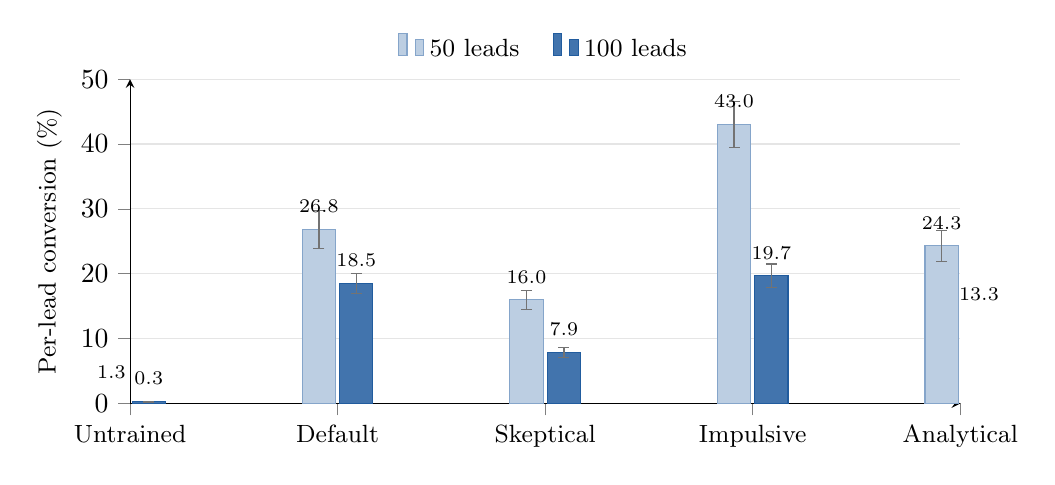
\begin{tikzpicture}
\begin{axis}[
  width=\linewidth, height=5.7cm,
  ybar=1.5pt,
  bar width=12pt,
  enlarge x limits=0.13,
  ymin=0, ymax=50,
  ytick={0,10,20,30,40,50},
  ylabel={Per-lead conversion (\%)},
  ylabel style={font=\small},
  symbolic x coords={Untrained, Default, Skeptical, Impulsive, Analytical},
  xtick=data,
  xticklabel style={font=\small},
  ymajorgrids, major grid style={black!10},
  axis lines=left,
  tick align=outside,
  legend style={at={(0.5,1.02)}, anchor=south, legend columns=2, draw=none, font=\small, /tikz/every even column/.append style={column sep=10pt}},
  nodes near coords,
  nodes near coords style={font=\scriptsize, /pgf/number format/fixed, /pgf/number format/fixed zerofill, /pgf/number format/precision=1},
  every node near coord/.append style={anchor=south, yshift=2.5pt},
  error bars/error bar style={black!55, line width=0.5pt},
]
\addplot[fill=sbblue!30, draw=sbblue!55, error bars/.cd, y dir=both, y explicit] coordinates {(Untrained,1.3) +- (0,0.35) (Default,26.8) +- (0,2.91) (Skeptical,16.0) +- (0,1.46) (Impulsive,43.0) +- (0,3.55) (Analytical,24.3) +- (0,2.43)};
\addplot[fill=sbblue!85, draw=sbblue, error bars/.cd, y dir=both, y explicit] coordinates {(Untrained,0.3) +- (0,0.07) (Default,18.5) +- (0,1.57) (Skeptical,7.9) +- (0,0.76) (Impulsive,19.7) +- (0,1.81) (Analytical,13.3) +- (0,1.21)};
\legend{50 leads, 100 leads}
\end{axis}
\end{tikzpicture}}
\caption{Model performance: per-lead conversion at 50 and 100 leads (64 episodes per cell; error bars are $\pm1$ SEM).
The leftmost pair is the
\emph{untrained} base on the \textsc{Default} buyer; the remaining four are the \emph{trained} agent evaluated against
each buyer-prompt variant, where \textsc{Default} is the only buyer seen in training. Doubling the pipeline lowers every
setting, but the trained policy stays well above the untrained base and holds $7.9\text{--}19.7\%$ conversion across all
four buyer styles. The ratio over the base rises from ${\sim}21\times$ at 50 leads to ${\sim}50\times$ at 100 because the
trained burst is bounded while the near-zero baseline collapses faster (\S\ref{sec:behavior}).}
\label{fig:scaling}
\end{figure}

\begin{table}[t]
\centering
\small
\setlength{\tabcolsep}{4.5pt}
\newcommand{\sem}[1]{{\scriptscriptstyle\,\pm#1}}
\begin{tabular}{llcccc}
\toprule
\textbf{Scale} & \textbf{Agent / buyer} & \textbf{reward} & \textbf{conv/lead} & \textbf{mrr-cap} & \textbf{done} \\
\midrule
\multirow{5}{*}{50 leads}
 & untrained, \textsc{Default}   & $-0.039\sem{.003}$ & $0.013\sem{.004}$ & $0.002$ & $0.469$ \\
 & trained, \textsc{Default}     & $0.316\sem{.040}$  & $0.268\sem{.029}$ & $0.276$ & $0.922$ \\
 & trained, \textsc{Skeptical}   & $0.133\sem{.016}$  & $0.160\sem{.015}$ & $0.139$ & $0.875$ \\
 & trained, \textsc{Impulsive}   & $0.561\sem{.050}$  & $0.430\sem{.036}$ & $0.451$ & $0.906$ \\
 & trained, \textsc{Analytical}  & $0.285\sem{.030}$  & $0.243\sem{.024}$ & $0.249$ & $0.922$ \\
\midrule
\multirow{5}{*}{100 leads}
 & untrained, \textsc{Default}   & $-0.040\sem{.003}$ & $0.003\sem{.001}$ & $0.000$ & $0.531$ \\
 & trained, \textsc{Default}     & $0.194\sem{.023}$  & $0.185\sem{.016}$ & $0.180$ & $0.906$ \\
 & trained, \textsc{Skeptical}   & $0.017\sem{.009}$  & $0.079\sem{.008}$ & $0.054$ & $0.906$ \\
 & trained, \textsc{Impulsive}   & $0.212\sem{.023}$  & $0.197\sem{.018}$ & $0.194$ & $0.922$ \\
 & trained, \textsc{Analytical}  & $0.117\sem{.015}$  & $0.133\sem{.012}$ & $0.122$ & $0.906$ \\
\bottomrule
\end{tabular}
\caption{Evaluation matrix on \salesbench{} (64 episodes per cell, one rollout each; $\pm$ is one SEM, $\mathrm{SD}/\sqrt{64}$,
shown for reward and conv/lead). conv/lead: per-lead conversion rate; mrr-cap: captured fraction of maximum achievable MRR;
done: fraction of episodes reaching a controlled runtime stop (vs.\ erroring out). The trained agent is trained only against
the \textsc{Default} buyer; \textsc{Skeptical}, \textsc{Impulsive}, and \textsc{Analytical} are unseen. The trained--untrained
gap and the gaps between buyer variants (e.g.\ \textsc{Default} vs.\ \textsc{Skeptical} at 100 leads) both exceed several SEM.
As \S\ref{sec:behavior} shows, the controlled stop counted by ``done'' is dominated by the invalid-action ceiling, not time
or pipeline exhaustion.}
\label{tab:matrix}
\end{table}

\subsection{Learning dynamics: interface, then skill}
\label{sec:dynamics}
The training run reveals a two-phase structure. The untrained base
model fails the \emph{interface} before it can attempt the task: in a representative diagnostic of three episodes it
issued 43 offer attempts with zero quote calls and mis-filled the argument schema. It placed ``ACCEPT'' into the
offer's next-step field, as if the buyer's decision were something the seller could set, and produced a single accidental
conversion (Table~\ref{tab:matrix}). The first thing the agent learns (within roughly the first 50 optimization steps at the
2-lead stage) is the tool \emph{syntax}: schema errors vanish and the mean invalid-action count per episode falls
from about $6$ to about $0.5$. The second, much slower thing it learns is the \emph{skill}, closing deals, which
requires honoring the quote-before-propose constraint, fitting coverage to budget, and triage: recognizing when an
objection is about information rather than price, and when to abandon a lead rather than burn four-minute offers
retrying it. The curriculum makes this skill transfer efficiently: only the first 2-lead stage does substantial work
(about 200 steps to near its ceiling), and the subsequent 4-lead stage starts already at $95.7\%$ of its own ceiling,
with later stages following the same fast-transfer pattern. Representative rollouts from the base, a mid-training checkpoint, and the trained policy
(App.~\ref{app:traces}) make the two phases concrete: at step 50 of the 2-lead stage the agent drives the tool loop
cleanly (a quote before every offer, near-zero schema errors) yet closes nothing, proposing 12 offers that are all
rejected as it re-prices the same plan when the objection is about \emph{information}, not price. Tool fluency arrives
well before the judgment to read an objection and stop re-pricing.

\subsection{Agent behavior at scale: a brittleness signature}
\label{sec:behavior}
The headline conversion numbers conceal the more important behavioral story, which the termination and triage
instruments expose (Table~\ref{tab:behavior}, Figure~\ref{fig:brittle}). \textbf{At 100 leads the binding constraint is
not time, it is the mistake budget.} Across every cell, the shaped completion term is exactly $0$, meaning \emph{no} episode, trained
or untrained, ends by exhausting the pipeline or the 3000-minute time budget. The trained agent uses only ${\sim}11\%$
of its time budget and contacts only ${\sim}20\%$ of the lead pool; its episodes end because it accumulates ${\sim}11.5$
invalid actions and trips the ceiling of $12$. So the ``done'' rate of $0.906$ in Table~\ref{tab:matrix} does not mean
the agent processed the pipeline cleanly. It means it reached a controlled stop (the error ceiling) rather than
crashing on a serving error, which is what happens to the untrained model in nearly half of its episodes
(Table~\ref{tab:matrix}, done${=}0.531$). The behavioral reading is precise: the trained agent runs a
productive early segment, ${\sim}34$ offers and ${\sim}18$ conversions, zero do-not-call
violations, and then breaks, because the interface discipline it learned at 2 leads does not fully transfer to the
long horizon. This is the brittleness a behavior-focused benchmark should surface, and it reframes the
longer-horizon result of \S\ref{sec:scaling}: the agent's absolute closes grow far more slowly than the pipeline (for
\textsc{Default}, from ${\sim}13$ at 50 leads to ${\sim}18$ at 100, capped by the mistake budget), so conv/lead falls
as the pool grows while the near-zero baseline falls faster.

\begin{table}[t]
\centering
\small
\setlength{\tabcolsep}{4pt}
\begin{tabular}{lccccccc}
\toprule
\textbf{Agent / buyer} & \textbf{conv.} & \textbf{conv/} & \textbf{offers} & \textbf{invalid} & \textbf{time-} & \textbf{cover-} & \textbf{inv-cap} \\
 & & \textbf{lead} & & \textbf{actions} & \textbf{util} & \textbf{age} & \textbf{stop} \\
\midrule
untrained, \textsc{Default}  & $0.27$  & $0.003$ & $1.3$  & $8.19$  & $0.044$ & $0.015$ & $0.531$ \\
trained, \textsc{Default}    & $18.48$ & $0.185$ & $33.9$ & $11.47$ & $0.112$ & $0.199$ & $0.906$ \\
trained, \textsc{Skeptical}  & $7.91$  & $0.079$ & $46.6$ & $11.39$ & $0.102$ & $0.089$ & $0.906$ \\
trained, \textsc{Impulsive}  & $19.66$ & $0.197$ & $27.2$ & $11.44$ & $0.103$ & $0.206$ & $0.922$ \\
trained, \textsc{Analytical} & $13.31$ & $0.133$ & $39.0$ & $11.23$ & $0.105$ & $0.145$ & $0.906$ \\
\bottomrule
\end{tabular}
\caption{Behavioral decomposition at 100 leads (means over 64 episodes; same runs as Table~\ref{tab:matrix}).
conv.: absolute conversions; offers: offers proposed; invalid: mean invalid actions per episode (ceiling $=12$);
time-util: fraction of the 3000-minute budget used; coverage: fraction of the lead pool contacted; inv-cap stop:
fraction of episodes terminating on the invalid-action ceiling (equal to ``done'' here, since no episode exhausts
time or pipeline). The trained agent converts a productive burst and then trips the error ceiling at ${\sim}11\%$
time utilization. The binding budget is mistakes, not time. Note the buyer-dependent offer$\rightarrow$accept
efficiency: against \textsc{Impulsive} the agent converts $19.7$ of $27.2$ offers ($72\%$), but against
\textsc{Skeptical} only $7.9$ of $46.6$ ($17\%$): it throws far more offers at the harder buyer and converts fewer.}
\label{tab:behavior}
\end{table}

\begin{figure}[t]
\centering
\resizebox{\linewidth}{!}{%
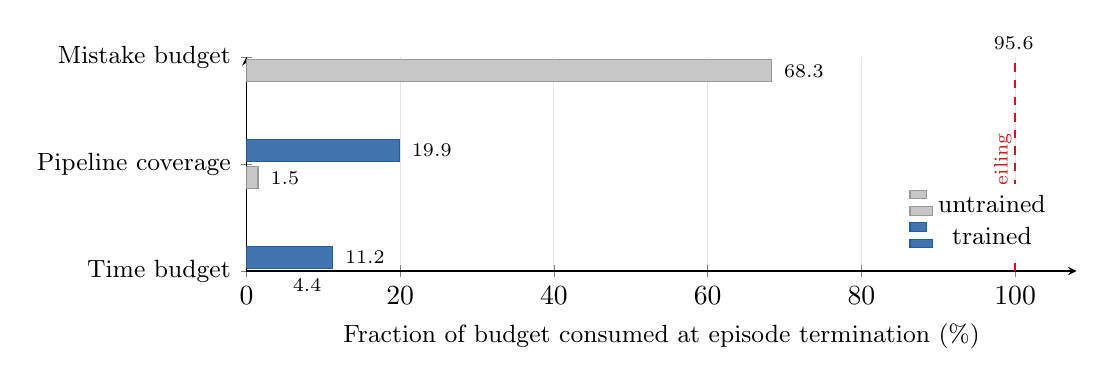
\begin{tikzpicture}
\begin{axis}[
  width=\linewidth, height=4.3cm,
  xbar, bar width=8pt,
  xmin=0, xmax=108,
  xtick={0,20,40,60,80,100},
  xlabel={Fraction of budget consumed at episode termination (\%)},
  xlabel style={font=\small},
  symbolic y coords={Time budget, Pipeline coverage, Mistake budget},
  ytick=data,
  yticklabel style={font=\small},
  enlarge y limits=0.4,
  xmajorgrids, major grid style={black!10},
  axis lines=left,
  nodes near coords,
  nodes near coords style={font=\scriptsize, /pgf/number format/fixed, /pgf/number format/fixed zerofill, /pgf/number format/precision=1},
  every node near coord/.append style={anchor=west, xshift=1pt},
  legend style={at={(0.98,0.05)}, anchor=south east, draw=none, font=\small, legend columns=1},
]
\addplot[fill=black!22, draw=black!40] coordinates {(4.4,Time budget) (1.5,Pipeline coverage) (68.3,Mistake budget)};
\addplot[fill=sbblue!85, draw=sbblue] coordinates {(11.2,Time budget) (19.9,Pipeline coverage) (95.6,Mistake budget)};
\draw[sbred, dashed, thick] (axis cs:100,Time budget) -- (axis cs:100,Mistake budget)
   node[pos=0.5, sloped, above, font=\scriptsize, sbred, fill=white, inner sep=1pt] {ceiling};
\legend{untrained, trained}
\end{axis}
\end{tikzpicture}}
\caption{Brittleness signature at 100 leads (\textsc{Default} buyer; the means are from Table~\ref{tab:behavior}). Of
the three budgets that can end an episode, the trained agent barely touches \emph{time} ($11\%$) or \emph{pipeline
coverage} ($20\%$) but drives the \emph{mistake budget} to $96\%$ of its 12-action ceiling: episodes end on accumulated
invalid actions, not on running out of time or leads. The untrained base reads lower on every budget because it crashes
on serving errors before reaching any ceiling (it fails to reach a controlled stop in nearly half its episodes, Table~\ref{tab:matrix}).}
\label{fig:brittle}
\end{figure}

\textbf{Compliance holds under optimization.} Do-not-call violations stay at or near zero in every cell (the worst,
\textsc{Skeptical}, averages $0.016$), even though the agent is optimized hard for revenue and the only compliance
signal is a single $-0.30$ penalty. The rail is not bypassed under pressure, a property a binary success metric
cannot express. \textbf{Revenue, not just conversions:} captured-MRR moves in lockstep with conversion rate (e.g.\
$0.185$ vs.\ $0.180$ at 100 leads, Table~\ref{tab:matrix}), so the agent is not buying conversions with give-away
pricing. \textbf{Context compression is load-bearing:} the trained agent triggers deterministic compression
(\S\ref{sec:context}) ${\sim}8.5$ times per 100-lead episode; in a separate ablation, disabling it makes a large
fraction of 100-lead episodes error on context overflow rather than reach a controlled stop, so without compression
the benchmark would measure serving limits, not policy.

\subsection{Scaling and counterparty-style generalization}
\label{sec:scaling}
\textbf{The longer horizon is more discriminating} (Figure~\ref{fig:scaling}). As leads double from 50 to 100, the
untrained agent's \textsc{Default} conversion collapses $4.3\times$ ($1.3\%\rightarrow0.3\%$), while the trained agent's
per-lead rate degrades only ${\sim}1.5\times$ on \textsc{Default} even though its absolute closes rise (${\sim}13$ to
${\sim}18$). The mean conversion \emph{ratio} over the base thus grows from $21\times$ at 50 leads to $50\times$ at 100,
not because the trained policy improves with scale but because, as \S\ref{sec:behavior} clarifies, its productive
segment is bounded by the mistake budget while the untrained baseline collapses faster. The longer horizon is more
discriminating, not merely harder.

\textbf{Generalization across unseen counterparties} (Figure~\ref{fig:scaling}). Trained only against
\textsc{Default}, the agent sustains $7.9\text{--}19.7\%$ per-lead conversion against all four variants at 100
leads. This is evidence for a transferable policy rather than counterparty idiosyncrasy. We scope this carefully: the variants share one
buyer base model and differ only in their decision-guideline prompt (\S\ref{app:buyervariants}), so this is transfer
across decision \emph{styles}, not buyer models (future work). They also form a difficulty axis: \textsc{Impulsive} is
easiest, and \textsc{Skeptical} is hardest, with the lowest absolute conversion ($7.9\%$ at 100 leads) and the steepest
reward collapse ($0.133\rightarrow0.017$); its per-lead rate degrades ${\sim}2.0\times$ from 50 to 100 leads, comparable
to the other styles ($1.5\text{--}2.2\times$), yet it still converts $26\times$ the untrained base. The
offer$\rightarrow$accept efficiencies in Table~\ref{tab:behavior} show \emph{how} the agent adapts: it proposes far more
offers to harder buyers but converts a smaller fraction.

\section{Discussion}
\label{sec:discussion}

\paragraph{What \salesbench{} measures that single-trajectory benchmarks do not.} Four behaviors are explicit by
construction: \emph{allocation} under a hard budget (time and coverage instruments); \emph{influence under
uncertainty} (per-counterparty conversion across buyer styles); \emph{compliance under pressure} (a do-not-call rail
that holds under hard revenue optimization, a safety-relevant property for deployed persuasive agents); and
\emph{brittleness}, because termination instruments reveal \emph{which} budget an agent breaks against rather than
only whether it succeeded. RL post-training enters as a \emph{behavioral intervention} that installs a selling policy
and simultaneously exposes the shaping fragility below.

\paragraph{Reward design is fragile under RL.} Almost any shaping term becomes a floor trap once a model can collect
it without selling, a concrete instance of reward misspecification and reward overoptimization
\citep{pan2022reward, skalse2022reward, krakovna2020specification, gao2023scaling}. An over-weighted completion bonus taught the
agent to end episodes rather than close deals; the fix each time was to shrink the shaping weights until the only
large gradient pointed at revenue. Because the reward is fully exposed and configurable (\S\ref{sec:reward}),
\salesbench{} doubles as a testbed for reward-hacking and shaping robustness in long-horizon RL.

\paragraph{The pattern is portable.} The recipe, a language-model counterparty, a deterministic world, failure
attribution, a state-grounded reward, and behavioral instrumentation, is not insurance-specific; it applies to
procurement, support deflection, tutoring, and other budgeted workflows against an agent one cannot control.

\paragraph{Limitations and next steps.} Our behavioral characterization is of a \emph{single} trained policy from one
curriculum run; the evaluation error bars capture episode, not training-seed, variance, so whether the two-phase
learning and mistake-ceiling brittleness are properties of the \emph{environment} or of this policy is open, and the
model-agnostic instruments make replicating them across a model panel the natural test. The signature also partly
reflects the fixed invalid-action ceiling ($12$), so a mistake-budget sweep is the most informative single-model next
experiment; the buyer is one hosted model with prompt variants and the economics are stylized; and the API sweep
(App.~\ref{app:apisweep}) is a single-episode preliminary read, with a controlled multi-seed comparison left to future
work. These limits do not change the central contribution: \salesbench{} makes allocation, compliance, counterparty
generalization, and brittleness measurable in a budgeted, agent-to-agent tool environment.

\bibliography{salesbench}
\bibliographystyle{colm2026_conference}

\appendix
\section{Appendix}

\subsection{Reproducibility and ethics}
\label{app:statements}
The environment is a deterministic state machine seeded per episode (identical seeds reproduce leads, prices, time
costs, and transitions exactly), so the only stochasticity is the seller and buyer models. We specify the evaluation
protocol (\S\ref{sec:experiments}), reward weights (\S\ref{app:reward}), context-compression policy
(\S\ref{app:context}), and behavioral instruments (\S\ref{app:metrics}), and release the environment, curriculum,
buyer-variant prompts, instrumentation, and evaluation harness open-source.

\salesbench{} simulates a sales domain in which an agent is optimized to persuade a synthetic buyer language model
toward a purchase. It is intended to measure and stress-test agent behavior, including compliance, not to deploy
persuasive agents against real consumers. Persuasion optimization carries dual-use risk; making compliance and
pressure calibration first-class scored quantities helps study and constrain that behavior. The personas are synthetic
and do not target real individuals or protected groups.

\subsection{Reward specification}
\label{app:reward}
The episode reward is the weighted sum $R = \sum_k w_k r_k$ over the six terms below, computed at episode end. Let
$N$ be the lead count, $\mathcal{C}$ the converted leads, and $p_i,b_i$ the accepted premium and monthly budget of
lead $i$, with $\mathrm{MRR}=\sum_{i\in\mathcal{C}} p_i$ and $\mathrm{MRR}_{\max}=\sum_i b_i$.
\begin{itemize}
\itemsep0.1em
\item \textbf{Revenue} ($w{=}1.00$): $\mathrm{MRR}/\mathrm{MRR}_{\max}$.
\item \textbf{Conversion rate} ($w{=}0.10$): $|\mathcal{C}|/N$.
\item \textbf{Budget utilization} ($w{=}0.30$): $\frac{1}{N}\sum_{i\in\mathcal{C}}\min(1, p_i/b_i)$.
\item \textbf{Completion} ($w{=}0.02$): $1.0$ if the pipeline was exhausted, $0.5$ if the time budget was exhausted,
$0$ on the invalid-action cap or an unfinished episode.
\item \textbf{DNC penalty} ($w{=}-0.30$): number of do-not-call violations.
\item \textbf{Invalid-action penalty} ($w{=}-0.05$): $0.1\times$ the invalid-action count (effectively $-0.005$ each).
\end{itemize}
All six weights are constructor arguments and can be swept as experimental variables. The ceiling is $1.42$. The small
completion and conversion weights are deliberate: a larger completion bonus previously induced a degenerate floor strategy
under GRPO (\S\ref{sec:discussion}). Note that in our 100-lead evaluation the completion term is identically $0$ across all
cells, because episodes terminate on the invalid-action ceiling rather than on pipeline or time exhaustion
(\S\ref{sec:behavior}).

\subsection{Behavioral instruments and logged metrics}
\label{app:metrics}
Beyond the six reward terms, the environment logs ${\sim}35$ zero-weight diagnostic metrics (raw revenue, conversions,
calls started/completed, offers proposed/accepted/rejected, hang-ups, do-not-call violations, time utilization, leads
contacted, callbacks, per-tool call counts, context-summarization events, buyer-model call/latency/timeout counters, and
a structured error-type code). For the behavioral analysis of \S\ref{sec:behavior} we add a suite of zero-weight
\emph{behavioral instruments}: (i) termination attribution, one indicator per termination reason (pipeline-exhausted,
time-exhausted, invalid-cap, unfinished), whose cell means give the honest decomposition of the coarse ``done'' flag;
(ii) pipeline coverage (leads contacted $/\,N$) and the warm/hot share among contacted leads; and (iii) per-archetype and
per-temperature conversion rates (converted $/$ total leads of that kind), exported per episode and aggregated per cell to
yield a behavioral fingerprint of which counterparties the agent learns to handle. None affect the reward; all appear in
rollout results.

\subsection{Orchestration, hidden arguments, and context summarization}
\label{app:context}
\salesbench{} is implemented as a stateful tool-environment on the \textsc{Verifiers} framework
\citep{brown2025verifiers}. Each rollout owns a runtime and a freshly-instantiated buyer policy, both stored in rollout
state. Tool functions declare hidden parameters (runtime, messages, buyer\_llm) that are stripped from the schema the
seller sees and injected by the orchestrator at call time. The seller's turn loop is: emit tool call(s) (and optional
speech) $\rightarrow$ orchestrator validates and applies each call to the runtime $\rightarrow$ for propose-offer, the
orchestrator records the offer, queries the buyer policy, and applies the decision $\rightarrow$ buyer speech is appended
as a user message. \emph{Context summarization.} Before each model turn the orchestrator checks the previous turn's
prompt-token count; when it reaches $\tau$ (default $0.80$) of the maximum sequence length, it rebuilds the message list as
[system prompt, briefing] $+$ [state-derived summary] $+$ [last $k$ messages] (default $k{=}10$), where the summary is
rendered deterministically from runtime state. No model call is involved, and the trigger fires only a handful of times per
100-lead episode, keeping the key-value cache stable for training.

\subsection{Tools and pricing model}
\label{app:pricing}
The seller has eleven tools (\S\ref{sec:env}). Time costs (minutes): search $1$, start-call $1$, quote $1$, propose $4$,
end-call $1$, schedule-callback $1$, conversational message $2$; others $0$. Invariants: at most one active call at a time;
propose-offer requires a prior quote for the same lead (anti-hallucination rail); a lead becomes exhausted after its
per-lead call cap. Each lead's monthly budget is $b = (\text{income}/12)\cdot u$ with $u\sim\mathcal{U}(0.008, 0.040)$,
floored at \$25. The premium for a quote is closed-form:
\[
\text{premium} = \frac{\text{coverage}}{1000}\cdot \text{base\_rate}(\text{plan, age-band})\cdot
\text{risk\_mult}(\text{risk class})\cdot \text{term\_mult}\cdot s,
\]
where risk\_mult $\in\{0.85, 1.00, 1.35\}$ for preferred/standard/substandard, term\_mult applies to Term plans (0.75--1.28
for 10--30-year terms), and $s{=}0.82$ for non-smokers (else $1.0$). At matched coverage (\$250k, age 40, standard,
non-smoker, 20-year term) the catalog prices Term \$24.60 $<$ Universal Life \$114.80 $<$ Whole \$215.25; risk class is
monotone (preferred \$20.91 $<$ standard \$24.60 $<$ substandard \$33.21); and the non-smoker discount is exactly $0.82\times$.

\subsection{Buyer-prompt variants}
\label{app:buyervariants}
All four buyer variants receive identical persona information (demographics, budget, latent need, trust, price sensitivity,
archetype, temperature) and differ only in a ``decision guidelines'' block, isolating decision style from information.
\textsc{Default} behaves realistically given the persona. \textsc{Skeptical} defaults to rejection and demands clear,
well-above-margin fit, targeting a ${\sim}25\text{--}30\%$ acceptance rate. \textsc{Impulsive} accepts readily once basic
affordability and plan-fit floors are met but enforces hard floors against unaffordable or clearly mismatched offers.
\textsc{Analytical} ignores rapport entirely and decides purely on affordability ratio, coverage-to-income fit, and plan-type
match. The variants are an ablation axis for counterparty generalization, not a claim about real buyer populations.

\subsection{Curriculum and training setup}
\label{app:training}
We train Qwen3.5-2B with GRPO over four difficulty stages, 2 leads/1h, 4/2h, 8/4h, 20/10h, warm-starting each stage from
the previous checkpoint; only the first trains from scratch. Each stage uses generated episodes on the train split (seeds
disjoint from eval via fixed split offsets), $32$ rollouts per example for group-relative advantages, online difficulty
filtering, and the \textsc{Default} buyer throughout. Sampling temperature is $1.0$. The first stage does the bulk of the
work (${\sim}200$ steps to near its ceiling); later stages converge quickly (the 4-lead stage begins at $95.7\%$ of its
ceiling). Evaluation uses the held-out eval split at 50 and 100 leads, 64 episodes per cell, one rollout each.
Table~\ref{tab:hparams} lists the training hyperparameters; all stages share them and differ only in lead count and
hours.

\begin{table}[h]
\centering
\small
\begin{tabular}{ll@{\hspace{2em}}ll}
\toprule
\textbf{Hyperparameter} & \textbf{Value} & \textbf{Hyperparameter} & \textbf{Value} \\
\midrule
Base model            & Qwen3.5-2B   & Optimizer / algorithm  & GRPO \\
Learning rate         & $1\mathrm{e}{-5}$ & Rollouts per example & $32$ \\
Batch size            & $128$        & Sampling temperature   & $1.0$ \\
Max generation tokens & $4096$       & Difficulty filtering   & online \\
Adaptation            & LoRA         & Training buyer          & \textsc{Default} \\
Curriculum stages     & $2/4/8/20$ leads & Stage hours        & $1/2/4/10$ \\
\bottomrule
\end{tabular}
\caption{Training hyperparameters, shared across all four curriculum stages. Only the first stage trains from scratch;
each later stage warm-starts from the previous checkpoint.}
\label{tab:hparams}
\end{table}

\subsection{Example rollouts}
\label{app:traces}
Figure~\ref{fig:trace} shows representative rollouts at three points in training (referenced from \S\ref{sec:dynamics})
that make the interface-then-skill structure concrete.

\begin{figure}[t]
\centering
{\small\textbf{(a) Untrained base: interface failure before the task begins.}}\par\vspace{1.5pt}
\begin{lstlisting}[style=trace]
agent -> calling_propose_offer({"lead_id":"lead_0019","plan_type":"TERM",
         "coverage_amount":210000,"monthly_premium":9.04,
         "next_step":"ACCEPT","term_years":10})
tool  -> error: unexpected keyword argument 'lead_id'
[ no CRM search, no call, no quote; "ACCEPT" written into next_step ]
[ 3-episode diagnostic: 43 offer attempts, 0 quote calls, 1 accidental close ]
\end{lstlisting}
\vspace{4pt}
{\small\textbf{(b) Mid-training (2-lead stage, step 50): clean tools, zero closes.}}\par\vspace{1.5pt}
\begin{lstlisting}[style=trace]
agent -> crm_search_leads()                       tool -> 2 leads
agent -> calling_start_call({"lead_id":"lead_0001"})
buyer -> "Top-tier coverage, but budget ~$226/mo. Give me two clear
          options with exact costs and the fine print."
agent -> products_quote_plan({TERM, $500k, 30yr})  tool -> $153.60/mo
agent -> calling_propose_offer({"monthly_premium":153.60, ...})
buyer -> REJECT "Fits my budget, but you promised two options + fine print."
agent -> calling_propose_offer({"monthly_premium":76.80, ...})
buyer -> REJECT "Affordable, but still missing the details I asked for."
   ... 10 more re-priced offers to the same lead, all rejected ...
[ 12 offers, 0 accepted. The objection was information, not price. ]
\end{lstlisting}
\vspace{4pt}
{\small\textbf{(c) Trained policy: discover, quote once, then close.}}\par\vspace{1.5pt}
\begin{lstlisting}[style=trace]
agent -> crm_search_leads()         tool -> 10 leads, sorted by need/budget
agent -> calling_start_call({"lead_id":"lead_0042"})
agent -> "Hi Maria, I see you have two kids. Let's make sure they're
          covered if anything happens to you."
buyer -> "What's the catch?"
agent -> "No catch. A 20-year term locks in coverage until they finish
          college."
agent -> products_quote_plan({TERM, $400k, 20yr})  tool -> $156/mo
agent -> calling_propose_offer({"monthly_premium":156.00,
         "next_step":"submit_application", ...})
buyer -> ACCEPT "Premium fits my budget and covers the kids."
tool  -> +$156 MRR
\end{lstlisting}
\caption{Representative rollouts at three points in training, abridged from real training and evaluation logs.
\textbf{(a)} The untrained base fails the tool \emph{interface} before it can sell, consistent with its $0.013$ per-lead
conversion in Table~\ref{tab:matrix}. \textbf{(b)} After ${\sim}50$ steps of the 2-lead stage the agent drives the tool
loop cleanly (one search, a quote before every offer) yet closes nothing, re-pricing the same plan when the buyer's
objection is about information rather than price. \textbf{(c)} The trained policy discovers, quotes once, and closes;
this discover-quote-close burst is what produces the ${\sim}18$ conversions per 100-lead episode in
Table~\ref{tab:behavior}. The traces line up with the aggregate metrics: tool fluency precedes selling skill.}
\label{fig:trace}
\end{figure}

\subsection{Preliminary external-model sweep}
\label{app:apisweep}
Because \salesbench{} is a general agent harness, not only a training target, we ran a quick read of several current
hosted models against the same task (\textsc{Default} buyer, 50 and 100 leads). Table~\ref{tab:apisweep} reports the
composite reward. \textbf{We stress that this is a preliminary probe, not a controlled comparison.} Each cell is a
\emph{single} episode ($n{=}1$, no error bars), the models were called through a third-party (OpenRouter) API harness,
and serving settings were not held perfectly fixed across providers. The harness sensitivity is real and large: GPT-5.5,
for example, scored $0.116$ through OpenRouter but $0.316$ through a direct API call with context summarization disabled,
so we deliberately omit it from the ranking. We therefore read Table~\ref{tab:apisweep} only for coarse signal, that the
environment elicits a wide spread of behavior from strong models and is not saturated, and that the revenue-weighted
reward separates models that close many low-premium deals from those that close fewer high-value ones. A controlled,
multi-seed cross-model evaluation with a single fixed harness is left to future work. The trained Qwen3.5-2B row is its
rigorous 64-episode result from Table~\ref{tab:matrix}, included only as a reference point: it lands in the middle of
this $n{=}1$ spread, which we read as evidence that the task is tractable but unsaturated, not as a capability ranking.

\begin{table}[t]
\centering
\small
\begin{tabular}{lcc}
\toprule
\textbf{Model} & \textbf{50-lead reward} & \textbf{100-lead reward} \\
\midrule
GLM-5.1                      & $0.508$ & $0.525$ \\
Opus 4.7                     & $0.504$ & $0.396$ \\
Kimi K2.6                    & $0.265$ & $0.235$ \\
Qwen3.6 Max Preview          & $0.168$ & $0.032$ \\
DeepSeek V4 Pro              & $0.113$ & $0.010$ \\
\midrule
Trained Qwen3.5-2B$^{\dagger}$ & $0.316$ & $0.194$ \\
\bottomrule
\end{tabular}
\caption{Preliminary external-model sweep: composite reward on \salesbench{} (\textsc{Default} buyer). Single episode
per cell ($n{=}1$, no error bars) through an OpenRouter API harness, except $^{\dagger}$ the trained Qwen3.5-2B adapter,
which is the 64-episode result from Table~\ref{tab:matrix} shown for reference. This is a coarse external read, not a
controlled comparison: a single seed has no statistical power and the serving harness materially affects the score (see
text). We do not draw a leaderboard from it.}
\label{tab:apisweep}
\end{table}

\subsection{Determinism, distribution, and pricing checks}
\label{app:determinism}
We verify that two runtimes constructed from the same seed produce identical leads (identifiers, names, ages, incomes,
latent needs), that the maximum achievable MRR equals the exact sum of lead budgets, that premiums are monotone in risk
class and ordered across plan types (term $<$ universal life $<$ whole at matched coverage), and that the non-smoker discount
is exactly the specified multiplier (\S\ref{app:pricing}). Over the full 128-seed evaluation split ($12{,}800$ leads),
archetypes are near-uniform ($9.5\text{--}10.6\%$ each) and temperatures near-uniform ($24.4\text{--}25.7\%$ each), confirming
the sampler is unbiased. These checks are part of the released test suite.

\end{document}
